\mysection[Salmon]{\centering Riemann Integral}
Seien $a,b\in\mathbb{R}, a<b$ und $I=[a, b]$.

\DEF{Partition}{Eine Partition von $I$ ist eine endliche Teilmenge $P\subsetneq[a,b]$ wobei $\{a,b\}\subseteq P$. Es gilt $n:=|P|-1\geq 1$ und $\exists$ genau eine Bijektion $\{0,...,n\}\rightarrow P, j\rightarrow x_j$ s.d. $i<j\Rightarrow x_i<x_j$.}

\DEF{Verfeinerung einer Partition}{Seien $P,P'$ Partitionen. Dann $P\subseteq P'\Rightarrow P'$ ist Verfeinerung von $P$.

Die Vereinigung $P_1\cup P_2$ zweier Partitionen ist wieder eine Partition, insbesondere haben zwei Partitionen immer eine gemeinsame Verfeinerung.}

\DEF{Untersumme \& Obersumme}{Sei $f:[a,b]\rightarrow\mathbb{R}$ s.d. $\exists M\geq 0$ mit $|f(x)|\leq M\ \forall x\in[a,b]$. Sei $P=\{x_0,...,x_n\}$ eine Partition von $I$ mit $x_0=a<x_1<...<x_n=b$. Sei $\delta_i:=x_i-x_{i-1}=|[x_{i-1},x_i]|, i\leq 1$. Dann ist 
\begin{enumerate}
    \item $s(f,P):=\sum_{i=1}^nf_i\delta_i$ wobei $f_i=inf_{x_{i-1}\leq x \leq x_i}f(x)$ die Untersumme, und
    \item $S(f,P):=\sum_{i=1}^nF_i\delta_i$ wobei $F_i=sup_{x_{i-1}\leq x \leq x_i}f(x)$ die Obersumme.
\end{enumerate}
Es gilt $-M\leq f_i\leq F_i\leq M \Rightarrow$ $-M(b-a)\leq s(f,P)\leq S(f,p)\leq M(b-a)$.

\begin{figure}[H]
 \centering
 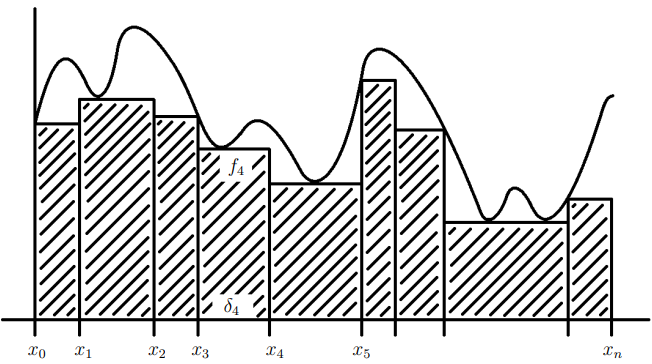
\includegraphics[width=\linewidth,keepaspectratio]{pictures/untersumme.png} 
\end{figure}

\begin{figure}[H]
 \centering
 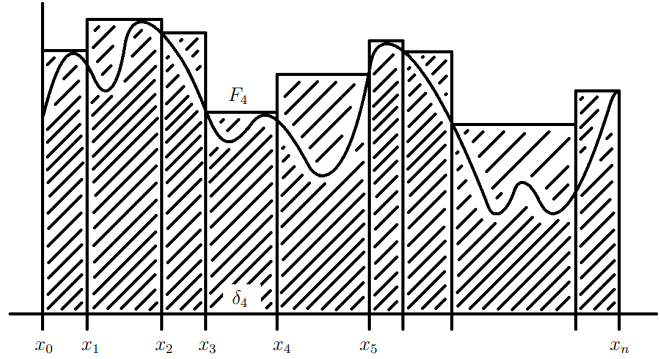
\includegraphics[width=\linewidth,keepaspectratio]{pictures/obersumme.png} 
\end{figure}}

\LEM{5.1.2}{
\begin{enumerate}
    \item Sei $P'$ eine Verfeinerung von $P$ $\Rightarrow$ $s(f,P)\leq s(f,P') \leq S(f,P') \leq S(f,P)$.
    \item Seien $P_1,P_2$ beliebige Partitionen $\Rightarrow$ $s(f,P_1)\leq S(f,P_2)$.
\end{enumerate}}

\DEF{Grösste Untersumme \& Kleinste Obersumme}{Sei $\mathcal{P}(I)$ die Menge aller Partitionen von $I$. Dann
\begin{enumerate}
    \item $s(f)=sup_{P\in\mathcal{P}(I)}s(f,P)$ die grösste Untersumme,
    \item $S(f)=inf_{P\in\mathcal{P}(I)}S(f,P)$ die kleinste Obersumme.
\end{enumerate}}

\COR{}{Aus L5.1.2 folgt $s(f)\leq S(f)$.}

\DEF{Integrierbarkeit}{Sei $f:[a.b]\rightarrow\mathbf{R}$ beschränkt. Dann $s(f)=S(f) \Rightarrow f$ ist (Riemann) integrierbar und wir definieren $\int_a^bf(x)dx:=s(f)=S(f)$.}

\SA{5.1.4}{Sei $f$ beschränkt. Dann $f$ integrierbar $\Leftrightarrow$ $\forall\varepsilon>0\ \exists P\in\mathcal{P}(I):S(f,P)-s(f,P)<\varepsilon$.}

\EXAMPLE{5.1.5}{Sei $f(x)=x$ auf $[a,b]$. Sei $P_n=\{a+i\cdot h:0\leq i\leq n\}$ wobei $h=\frac{b-a}{n}$. Dann $s(f,P_n)=\sum_{i=1}^nx_{i-1}(x_i-x_{i-1})=(b-a)a+\frac{(b-a)^2}{2}(\frac{n-1}{n})$ und $S(f,P_n)=\sum_{i=1}^nx_{i}(x_i-x_{i-1})=(b-a)a+\frac{(b-a)^2}{2}(\frac{n+1}{n})$. Somit $lim_{n\rightarrow\infty}s(f,P_n)=S(f,P_n)=\frac{b^2-a^2}{2}$ $\Rightarrow$ $f$ integrierbar $\land$ $\int_a^bf(x)dx=\frac{b^2-a^2}{2}$.}

\EXAMPLE{5.1.6}{Sei $f:[0,1]\rightarrow\mathbb{R}$ definiert durch $f(x)=\begin{cases}
    1 & \text{$x$ rational}\\
    0 & \text{$x$ irrational}.
\end{cases}$

Es folgt $s(f,P)=0\not = 1 = S(f,P)\ \forall P\in\mathcal{P}(I)$ $\Rightarrow f$ nicht integrierbar.}

\EXAMPLE{5.1.7}{Sei $f:[0,1]\rightarrow\mathbb{R}$ definiert durch $f(x)=\begin{cases}
    0 & \text{$x$ irrational $\lor\ x= 0$},\\
    \frac{1}{q} & \text{$x=\frac{p}{q},p,q\in\mathbb{N},gcd(p,q)=1$}.
\end{cases}$

Dann $f$ integrierbar und $\int_0^1f(x)dx=0$.}

\SA{5.1.8 (Du Bois-Reymond 1875, Darboux 1875)}{Sei $f$ beschränkt. Dann $f$ integrierbar $\Leftrightarrow$ $\forall\varepsilon>0\ \exists \delta > 0:\forall P\in\mathcal{P}_{\delta}(I), S(f,P)-s(f,P)<\varepsilon$. $\mathcal{P}_{\delta}(I)$ bezeichnet die Menge aller Partitionen $P$ mit $max_{1\leq i\leq n}\delta_i\leq\delta$.}

\DEF{Notation}{Sei $P=\{x_0,...,x_n\}$ eine Partition. Dann $\delta(P):=max_{1\leq i\leq n}(x_i-x_{i-1})$.}

\DEF{Riemannsche Summe}{Sei $\xi_1,...,\xi_n:\xi_i\in[x_{i-1},x_i], 1\leq i \leq n$. Dann ist $\sigma:=\sum_{i=1}^nf(\xi_i)\delta_i$ eine Riemannsche Summe.}

\COR{5.1.9}{Sei $f$ beschränkt. Dann $f$ integrierbar mit $A:=\int_a^bf(x)dx \Leftrightarrow$ $\forall\varepsilon > 0\ \exists\delta > 0:\ \forall P\in\mathcal{P}(I)$ mit $\delta(P)<\delta$ $\land$ $\xi_1,...\xi_n$ mit $\xi_i\in[x_{i-1},x_i],P=\{x_0,...,x_n\},$ $|A-\sum_{i=1}^nf(\xi_i)(x_i-x_{i-1})|<\varepsilon$.}

\mysubsection{Integrierbare Funktionen}
\SA{5.2.1}{Seien $f,g:[a,b]\rightarrow\mathbb{R}$ beschränkt, integrierbar und $\lambda\in\mathbb{R}$. Dann sind $f+g,\lambda\cdot f,f\cdot g,|f|,max(f,g),min(f,g)$ und $\frac{f}{g}$ (falls $|g(x)|\geq\beta > 0\ \forall x\in[a,b]$) integrierbar.}

\NOTE{5.2.2}{Sei $\phi[c,d]\rightarrow\mathbb{R}$ beschränkt. Dann $sup_{x,y\in[c,d]}|\phi(x)-\phi(y)|=sup_{x\in[c,d]}\phi(x)-inf_{x\in[c,d]}\phi(x)$.}

\COR{5.2.3}{Seien $P,Q$ Polynome und $[a,b]$ ein Intervall s.d. $\forall x\in[a,b]:Q(x) \not= 0$. Dann ist $[a,b]\rightarrow\mathbb{R}, x\mapsto\frac{P(x)}{Q(x)}$ integrierbar.}

\DEF{Gleichmässige Stetigkeit}{Sei $f:D\rightarrow\mathbb{R}, D\subseteq\mathbb{R}$. $\forall\varepsilon > 0\ \exists\delta>0\ \forall x,y\in D: (|x-y|<\delta\Rightarrow|f(x)-f(y)|<\varepsilon)$ $\Rightarrow$ $f$ in $[a,b]$ gleichmässig stetig.}

\EXAMPLE{5.2.5}{$f:\mathbb{R}\rightarrow\mathbb{R}, x\mapsto x^2$ ist auf $\mathbb{R}$ stetig aber nicht gleichmässig stetig.}

\SA{5.2.6 (Heine 1872)}{Sei $f:[a,b]\rightarrow\mathbb{R}$ stetig in dem kompakten Intervall $[a,b]$. Dann ist $f$ in $[a,b]$ gleuchmässig stetig.}

\SA{5.2.7/8}{Sei $f:[a,b]\rightarrow\mathbb{R}$. 
\begin{enumerate}
    \item $f$ stetig $\Rightarrow$ $f$ integrierbar.
    \item $f$ monoton $\Rightarrow$ $f$ integrierbar.
\end{enumerate}}

\NOTE{5.2.9}{Seinen $a<b<c$ und $f:[a,c]\rightarrow\mathbb{R}$ beschränkt. 
\begin{enumerate}
    \item $f|_{[a,b]}$ und $f|_{[b,c]}$ integrierbar $\Rightarrow f$ integrierbar $\land$ $\int_a^cf(x)dx=\int_a^bf(x)dx+\int_b^cf(x)dx$.
    \item $\int_a^af(x)dx=0$.
    \item $\int_b^af(x)dx:=-\int_a^bf(x)dx$ falls $a<b$.
\end{enumerate}}

\SA{5.2.10 (Linearität)}{Sei $I\subsetneq\mathbb{R}, I=[a,b]$. Seien $f_1,f_2:I\rightarrow\mathbb{R}$ beschränkt integrierbar. Seien $\lambda_1,\lambda_2\in\mathbb{R}$. Dann $\int_a^b(\lambda_1f_1(x)+\lambda_2f_2(x))dx=\lambda_1\int_a^bf_1(x)dx+\lambda_2\int_a^bf_2(x)dx$.}

\mysubsection{Ungleichungen und Mittelwertsatz}
\SA{5.3.1 (Monotonie)}{Seien $f,g:[a,b]\rightarrow\mathbb{R}$ beschränkt integrierbar.

$f(x)\leq g(x)\ \forall x\in[a,b]$ $\Rightarrow$ $\int_a^bf(x)dx\leq\int_a^bg(x)dx$.}

\COR{5.3.2 (Dreiecksungleichung)}{$f:[a,b]\rightarrow\mathbb{R}$ beschränkt integrierbar $\Rightarrow$ $|\int_a^bf(x)dx|\leq\int_a^b|f(x)|dx$.}

\SA{5.3.3 (Cauchy-Schwarz Ungleichung)}{$f,g:[a,b]\rightarrow\mathbb{R}$ beschränkt integrierbar $\Rightarrow$ $|\int_a^bf(x)g(x)dx|\leq \sqrt{\int_a^bf^2(x)dx}\sqrt{\int_a^bg^2(x)dx}$.}

\SA{5.3.4 (Mittelwertsatz)}{$f:[a,b]\rightarrow\mathbb{R}$ stetig $\Rightarrow$ $\exists\xi\in[a,b]$ mit $\int_a^bf(x)dx=f(\xi)(b-a)$.}

\EXAMPLE{5.3.5}{Sei $f:[0,1]\rightarrow\mathbb{R}, f(x)=\begin{cases}
    0 & 0\leq x < \frac{1}{2},\\
    1 & \frac{1}{2} \leq x \leq 1.
\end{cases}$

Dann ist $\int_0^1f(x)dx=\int_0^{\frac{1}{2}}\textbf{0}dx+\int_{\frac{1}{2}}^1\textbf{1}dx=\frac{1}{2}$.}

\SA{5.3.6 (Cauchy 1821)}{Seien $f,g:[a,b]\rightarrow\mathbb{R}$ wobei $f$ stetig, $g$ beschränkt integrierbar mit $g(x)\geq 0\ \forall x\in[a,b]$. Dann $\exists\xi\in[a,b]$ mit $\int_a^bf(x)g(x)dx=f(\xi)\int_a^bg(x)dx$.}

\mysubsection{Fundamentalsatz Differentialrechnung}
\SA{5.4.1}{Seien $a<b, f:[a,b]\rightarrow\mathbb{R}$ stetig. $F(x)=\int_a^xf(t)dt, a\leq x\leq b$ ist in $[a,b]$ stetig differenzierbar und $F'(x)=f(x)\ \forall x\in[a,b]$.}

\DEF{Stammfunktion}{Sei $a<b,f:[a,b]\rightarrow\mathbb{R}$ stetig. Sei $F:[a,b]\rightarrow\mathbb{R}$. $F$ (stetig) differenzierbar in $[a,b]$ $\land$ $F'=f$ in $[a,b]$ $\Rightarrow$ $F$ Stammfunktion von $f$.}

\SA{5.4.3 (Fundamentalsatz Differentialrechnung)}{$f:[a,b]\rightarrow\mathbb{R}$ stetig $\Rightarrow$ $\exists$ $F:F'=f$, $F$ bis auf additive Konstante eindeutig bestimmt $\land$ $\int_a^bf(x)dx=F(b)-F(a)$.}

\EXAMPLE{5.4.4}{
\begin{enumerate}
    \item $f(x)=x$. Dann $F(x)=\frac{x^2}{2}\Rightarrow\int_0^af(x)dx=\int_0^axdx=F(a)-F(0)=\frac{a^2}{2}$.
    \item $f(x)=x^2$. Dann $F(x)=\frac{x^3}{3}\Rightarrow\int_0^af(x)dx=\int_0^ax^2dx=F(a)-F(0)=\frac{a^3}{3}$.
\end{enumerate}}

\SA{5.4.5 (Partielle Integration)}{Seien $a,b\in\mathbb{R}, a<b$. Seien $f,g:[a,b]\rightarrow\mathbb{R}$ stetig differenzierbar. Dann $\int_a^bf(x)g'(x)dx=f(b)g(b)-f(a)g(a)-\int_a^bf'(x)g(x)dx$.}

\SA{5.4.6 (Substitution)}{Sei $a<b, \phi:[a,b]\rightarrow\mathbb{R}$ stetig differenzierbar, $I\subseteq\mathbb{R}$ mit $\phi([a,b])\subseteq I$ und $f:I\rightarrow\mathbb{R}$ stetig. Dann $\int_{\phi(a)}^{\phi(b)}f(x)dx=\int_a^bf(\phi(t))\phi'(t)dt$.}

\EXAMPLE{5.4.7}{
\begin{enumerate}
    \item Sei $f:[a,b]\rightarrow[0,\infty)$ beschränkt integrierbar. Dann ist der Flächeninhalt unter der Kurve $f$ definiert als $\{(x,y)\in\mathbb{R}^2:a\leq x\leq b, 0\leq y\leq f(x)\}:=\int_a^bf(t)dt$.
    \item Sei $f(x)=c\in\mathbb{R}$. Dann $\int_a^bf(x)dx=c\cdot\int_a^b\textbf{1}dx=c(b-a)$.
    \item .
\end{enumerate}}

\COR{5.4.8}{Sei $I\subseteq\mathbb{R}$. Sei $f:I\rightarrow\mathbb{R}$ stetig.
\begin{enumerate}
    \item $a,b,c\in\mathbb{R}:[a+c,b+c]\subseteq I$ $\Rightarrow$ $\int_{a+c}^{b+c}f(x)dx=\int_a^bf(t+c)dt$.
    \item $a,b,c\in\mathbb{R},c\not=0:[ac,bc]\subseteq I$ $\Rightarrow$ $\frac{1}{c}\int_{ac}^{bc}f(x)dx=\int_{a}^{b}f(ct)dt$.
\end{enumerate}}

\mysubsection{Integration konvergenter Reihen}
\SA{5.5.1}{$f_n:[a,b]\rightarrow\mathbb{R}$ beschränkt integrierbar und gleichmässig konvergent gegen $f:[a,b]\rightarrow\mathbb{R}$ $\Rightarrow$ $f$ beschränkt integrierbar $\land$ $lim_{n\rightarrow\infty}\int_a^bf_n(x)dx=\int_a^bf(x)dx$.}

\COR{5.5.2}{$f_n:[a,b]\rightarrow\mathbb{R}$ beschränkt integrierbar s.d. $\sum_{n=0}^{\infty}f_n$ auf $[a,b]$ gleichmässig konvergiert. Dann $\sum_{n=0}^{\infty}\int_a^bf_n(x)dx=\int_a^b(\sum_{n=0}^{\infty}f_n(x))dx$.}

\COR{5.5.3}{Sei $f(x)=\sum_{n=0}^{\infty}c_nx^n$ eine Potenzreihe mit $\rho > 0$. Dann $\forall 0\leq r < \rho:f$ auf $[-r,r]$ integrierbar $\land\ \forall x\in(-\rho,\rho):$ $\int_0^xf(t)dt=\sum_{n=0}^{\infty}\frac{c_n}{n+1}x^{n+1}$.}

\EXAMPLE{5.5.4}{$ln(2)=1-\frac{1}{2}+\frac{1}{3}-\frac{1}{4}+...$}

\EXAMPLE{5.5.5}{$\frac{\pi}{4}=1-\frac{1}{3}+\frac{1}{5}-\frac{1}{7}+...$}

\mysubsection{Euler-McLaurin Summationsformel}
Sei $P_0 = 1$. Sei $P_1,P_2,...,P_k,...$ eine Folge von Polynomen die eindeutig durch folgende Eigenschaften bestimmt ist \begin{enumerate}
    \item $P'_k=P_{k-1}\ \forall k\geq 1$.
    \item $\int_0^1P_k(x)dx=0\ \forall k\geq 1$.
\end{enumerate}

Es gilt also $P_k(x)=\int_0^xP_{k-1}(t)dt+C$ und $\int_0^1\int_0^xP_{k-1}(t)dt\ dx+C=0$. Damit sind $C$ und $P_k$ eindeutig bestimmt.

\DEF{Bernoulli Polynom}{Das k'te Bernoulli Polynom ist $B_k(x)=k!P_k(x)\ \forall k\geq 0$. Also $B_0(x)=1$,  $B_1(x)=x-\frac{1}{2}$,  $B_2(x)=x^2-x+\frac{1}{6}$, $...$}

\DEF{5.6.2}{Sei $B_0=1$. $\forall k\geq 2$ definieren wir rekursiv $\sum_{i=0}^{k-1} {k\choose i}B_i=0$. Also $B_0=1$, $B_0+2B_1=0$, $B_0+3B_1+3B_2=0$, $...$}

\SA{5.6.3}{$B_k(x)=\sum_{i=0}^k{k\choose i}B_ix^{k-i}$.}

\NOTE{5.6.4}{Für $k\geq 2:B_k(1)=\sum_{i=0}^k{k\choose i}B_i=\sum_{i=0}^{k-1}{k\choose i}B_i+B_k=B_k=B_k(0)$.}

\DEF{Summationsformel}{Für $k\geq 1:\tilde{B}_k:[0,\infty)\rightarrow\mathbb{R}$, $\tilde{B}_k(x)=\begin{cases}
    B_k(x) & 0\leq x\leq 1,\\
    B_k(x-n) & n\leq x < n+1, n\geq 1.
\end{cases}$}

$\tilde{B}_1:$
\begin{figure}[H]
 \centering
 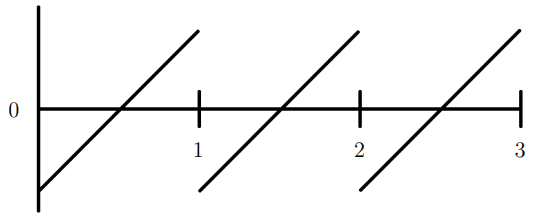
\includegraphics[width=\linewidth,keepaspectratio]{pictures/bernoulli_polynom.png} 
\end{figure}

\SA{5.6.5}{Sei $f:[0,n]\rightarrow\mathbb{R}$ $k$-mal stetig differenzierbar, $k\geq 1$. Dann
\begin{enumerate}
    \item Für $k=1:\sum_{i=1}^nf(i)=\int_0^nf(x)dx+\frac{1}{2}(f(n)-f(0))+\int_0^n\tilde{B}_1(x)f'(x)dx$.
    \item Für $k\geq 2:\sum_{i=1}^nf(i)=\int_0^nf(x)dx+\frac{1}{2}(f(n)-f(0))+\sum_{j=2}^k\frac{(-1)^jB_j}{j!}(f^{(j-1)}(n)-f^{(j-1)}(0))+\tilde{R}_k$ wobei $\tilde{R}_k=\frac{(-1)^{k-1}}{k!}\int_0^k\tilde{B}_k(x)f^{(k)}(x)dx$.
\end{enumerate}}

\NOTE{5.6.6}{
\begin{enumerate}
    \item $f(x):=\sum_{n=0}^{\infty}\frac{B_n}{n!}x^n=1-\frac{x}{2}+\frac{1}{6}\frac{x^2}{2!}+...=\frac{x}{e^x-1}$.
    \item $B_{2n+1}=0\ \forall n\geq 1$.
\end{enumerate}}

\NOTE{5.6.7}{Einfachste Anwendung der Euler-McLaurin Summationsformel. Sei $f(x)=x^l$, $l\geq 1, l\in\mathbb{N}$, $k=l+1$. Dann $\forall l\geq 1:1^l+...+n^l=\frac{1}{l+1}\sum_{j=0}^l(-1)^jB_j{l+1\choose j}n^{l+1-j}$.}


\mysubsection{Stirling'sche Formel}
\DEF{Stirling'sche Formel}{$n!\approx\frac{\sqrt{2\pi n}n^n}{e^n}$. Das heisst $lim_{n\rightarrow\infty}\frac{n!}{\frac{\sqrt{2\pi n}n^n}{e^n}}=1.$}

\SA{5.7.1}{$n!=\frac{\sqrt{2\pi n}n^n}{e^n}\cdot exp(\frac{1}{12n}+R_3(n))$ wobei $|R_3(n)|\leq\frac{\sqrt{3}}{216}\cdot\frac{1}{n^2}\ \forall n\geq 1$.}

\LEM{5.7.2}{$\forall m\geq n+1\geq 1:|R_3(m,n)|\leq\frac{\sqrt{3}}{216}(\frac{1}{n^2}-\frac{1}{m^2})$.}


\mysubsection{Uneigentliche Integrale}
\DEF{Grenzwert von Integralen}{Sei $f:[a,\infty)\rightarrow\mathbb{R}$ beschränkt, integrierbar auf $[a,b]\ \forall b>a$. Falls $\exists\ lim_{b\rightarrow\infty}\int_a^bf(x)dx \Rightarrow lim_{b\rightarrow\infty}\int_a^bf(x)dx:=\int_a^{\infty}f(x)dx$ $\land\ f$ auf $[a,\infty)$ integrierbar.}

\EXAMPLE{5.8.2}{
\begin{enumerate}
    \item $\int_0^{\infty}e^{-x}dx=lim_{b\rightarrow\infty}\int_0^be^{-x}dx=lim_{b\rightarrow\infty}(1-e^{-b})=1$.
    \item $\int_1^b\frac{1}{x^a}dx=\begin{cases}
    ln(b) & \alpha = 1,\\
    \frac{b^{1-\alpha}-1}{1-\alpha} & \alpha\not = 1.
\end{cases}$ Somit: $\int_1^{\infty}\frac{1}{x^a}dx=\begin{cases}
    divergiert & \alpha\leq 1,\\
    \frac{1}{\alpha-1} & \alpha > 1.
\end{cases}$
\end{enumerate}}

\LEM{5.8.3 (Vergleichssatz)}{Sei $f:[a,\infty)\rightarrow\mathbb{R}$ beschränkt, integrierbar auf $[a,b]\ \forall b>a$.
\begin{enumerate}
    \item Falls $|f(x)|\leq g(x)\ \forall x\geq a$ $\land\ g(x)$ auf $[a,b]$ integrierbar $\Rightarrow$ $f$ auf $[a,\infty)$ integrierbar.
    \item Falls $0\leq g\leq f$ $\land$ $\int_a^{\infty}g(x)dx$ divergiert $\Rightarrow$ $\int_a^{\infty}f(x)dx$ divergiert.
    \item Falls $0\leq |f|\leq g$ $\land$ $\int_a^{\infty}g(x)dx$ konvergiert $\Rightarrow$ $\int_a^{\infty}f(x)dx$ konvergiert.
\end{enumerate}}

\EXAMPLE{5.8.4}{Sei $\alpha > 0$. $\int_1^{\infty}\frac{1}{1+x^a}dx$ konvergiert für $\alpha > 1$, divergiert für $\alpha \leq 1$.}

\SA{5.8.5 (McLaurin 1742)}{Sei $f:[1,\infty)\rightarrow[0,\infty)$ monoton fallend. 

$\sum_{n=1}^{\infty}f(n)$ konvergiert $\Leftrightarrow$ $\int_1^{\infty}f(x)dx$ konvergiert.}

\EXAMPLE{5.8.6}{Für $\alpha > 1:$ $\sum_{n=2}^{\infty}\frac{1}{n^a}\leq\int_1^{\infty}\frac{1}{x^a}dx=\frac{1}{\alpha-1}\leq\sum_{n=1}^{\infty}\frac{1}{n^a}\leq\frac{\alpha}{\alpha-1}$.}

\EXAMPLE{5.8.7}{Sei $\beta > 0$. $\sum_{n=2}^{\infty}\frac{1}{n(ln(n))^{\beta}}$ konvergiert $\Leftrightarrow$ $\int_{2}^{\infty}\frac{1}{x(ln(x))^{\beta}}dx$ konvergiert $\Leftrightarrow$ $\beta > 1$.}

\DEF{Uneigentliches Integral}{Sei $f:(a,b]\rightarrow\mathbb{R}$. Falls $\exists \lim_{\varepsilon\rightarrow 0^+}\int_{a+\varepsilon}^bf(x)dx$ $\Rightarrow$ $f$ integrierbar $\land$ $\lim_{\varepsilon\rightarrow 0^+}\int_{a+\varepsilon}^bf(x)dx:=\int_a^bf(x)dx$.}

\EXAMPLE{5.8.9}{Sei $\frac{1}{x^a},x\in(0,1]$. Dann für $\varepsilon > 0:\int_{\varepsilon}^1\frac{1}{x^a}dx=\begin{cases}
    -ln(\varepsilon) & \alpha = 1,\\
    \frac{1-\varepsilon^{1-\alpha}}{1-\alpha} & \alpha\not = 1.
\end{cases}$

Somit $\int_0^1\frac{1}{x^a}dx=\begin{cases}
    divergiert & \alpha \geq 1,\\
    \frac{1}{1-\alpha} & \alpha < 1.
\end{cases}$}

\DEF{Gamma Funktion}{$\Gamma:(0,\infty)\rightarrow(0,\infty)$, $\Gamma(n):=\int_0^{\infty}e^{-x}x^{n-1}dx=(n-1)!$.}

\SA{5.8.12 (Bohr-Mollerup)}{
\begin{enumerate}
    \item $\Gamma$ erfüllt die Relationen
    \begin{enumerate}
        \item $\Gamma(1)=1$
        \item $\Gamma(n+1)=n\Gamma(n)\ \forall n > 0$
        \item $\Gamma$ logarithmisch konvex $\Leftrightarrow$ $\Gamma(\lambda x+(1-\lambda)y)\leq\Gamma(x)^{\lambda}\Gamma(y)^{1-\lambda}\ \forall x,y>0,\ 0\leq\lambda\leq 1$.
    \end{enumerate}
    \item $\Gamma$ ist die einzige Funktion $(0,\infty)\rightarrow(0,\infty)$ die a), b), c) erfüllt.
    \item $\Gamma(x)=lim_{n\rightarrow\infty}\frac{n!n^x}{x(x+1)...(x+n)}\ \forall x>0$.
\end{enumerate}}

\DEF{Young'sche Ungleichung}{Sei $\phi:[0,\infty)\rightarrow[0,\infty)$ stetig, strikt monoton wachsend, bijektiv mit $\phi(0)=0$. Seien $a,b\geq 0$. Dann $a\cdot b\leq\int_0^a\phi(x)dx+\int_0^b\phi^{-1}(y)dy$.}

\begin{figure}[H]
 \centering
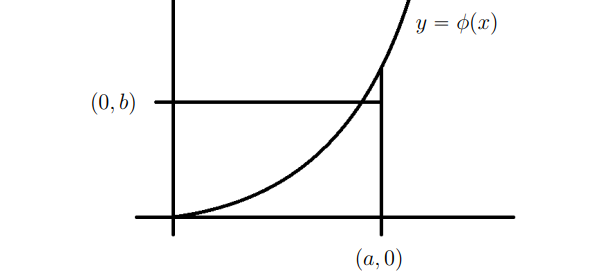
\includegraphics[width=\linewidth,keepaspectratio]{pictures/youngsche_ungleichung.png} 
\end{figure}

\LEM{5.8.13}{Seien $p> 1,\ q>1$ mit $\frac{1}{p}+\frac{1}{q}=1$. Dann $\forall a,b\geq 0:a\cdot b\leq\frac{a^p}{p}+\frac{b^q}{q}$.}

\DEF{Def}{Sei $a<b$, $p>1$. Für $f:[a,b]\rightarrow\mathbb{R}$ ist $||f||_p:=(\int_a^b|f(x)|^pdx)^{\frac{1}{p}}$. Es gilt $||f||_p=0\Leftrightarrow f=0$.}

\SA{5.8.14 (Hölder Ungleichung)}{Seien $p> 1,\ q>1$ mit $\frac{1}{p}+\frac{1}{q}=1$. Dann $\forall\ f,g:[a,b]\rightarrow\mathbb{R}$ stetig gilt $\int_a^b|f(x)g(x)|dx\leq ||f||_p||g||_q$.}

\mysubsection{Unbestimmte Integrale}
Sei $I\in\mathbb{R}$. Falls $f$ stetig $\Rightarrow$ $\exists$ Stammfunktion $F$ für $f$ (S 5.4.1) und $\int f(x)dx=F(x)+C$. Die Integrationskonstante $C$ deutet an, dass wir jede andere Stammfunktion durch addieren einer beliebigen Konstanten erhalten können.

\EXAMPLE{}{
\begin{enumerate}
    \item $\int x^sdx=\begin{cases}
    \frac{x^{s+1}}{s+1}+C & s\not =-1,\\
    ln(x)+C & x>0.
    \end{cases}$
    \item $\int e^xdx=e^x+C$.
    \item $\int sin(x)dx=-cos(x)+C$.
    \item $\int cos(x)dx=sin(x)+C$.
    \item $\int sinh(x)dx=cosh(x)+C$.
    \item $\int cosh(x)dx=sinh(x)+C$.
    \item $\int\frac{1}{\sqrt{1-x^2}}dx=arcsin(x)+C$.
    \item $\int\frac{1}{1+x^2}dx=arctan(x)+C$.
    \item $\int\frac{1}{\sqrt{1+x^2}}dx=arsinh(x)+C$.
    \item $\int\frac{1}{\sqrt{x^2-1}}dx=arcosh(x)+C$.
\end{enumerate}}

\DEF{Partielle Integration}{$\int f\cdot g'=f\cdot g-\int f'\cdot g$.}

\DEF{Substitution}{Sei $F(x)=\int f(x)dx$. Sei $x=\phi(u)$. Dann $F\circ\phi(u)=\int f(\phi(u))\phi'(u)du$.}

\EXAMPLE{5.9.1 (Partielle Integration)}{
\begin{enumerate}
    \item $\int ln(x)\cdot1 dx=xln(x)-\int\frac{1}{x}xdx=xln(x)-\int 1dx=xln(x)-x$.
    \item $\int x ln(x)dx=\frac{x^2}{2}ln(x)-\frac{1}{2}\int xdx=\frac{x^2}{2}ln(x)-\frac{x^2}{4}$.
    \item $\int x^2sin(x)dx=-x^2cos(x)+\int 2xcos(x)dx=-x^2cos(x)+2xsin(x)+2xcos(x)$.
    \item Sei $n\geq 1$. Dann $I_n=\int sin^n(x)dx=-\frac{1}{n}cos(x)sin^{n-1}x+\frac{n-1}{n}I_{n-2}$. Falls $n$ gerade $I_0=\int dx=x$. Falls $n$ ungerade $I_1=\int\sin(x)dx=-cos(x)$.
    \item $J_n=\int\frac{1}{(1+x^2)^n}dx=\frac{x}{(1+x^2)^n}+2nJ_n-2nJ_{n+1}$ $\Leftrightarrow$ $J_{n+1}=\frac{1}{2n}\frac{x}{(1+x^2)^n}+(\frac{2n-1}{2n})J_n$ 
$J_1=\int\frac{1}{1+x^2}dx=arctan(x)$.
\end{enumerate}}

\EXAMPLE{5.9.2 (Substitution)}{
\begin{enumerate}
    \item Sei $\int\frac{1}{a^2+x^2}dx$. Wähle $x=au\Rightarrow dx=a\cdot du$. Dann $\int\frac{1}{a^2+x^2}dx=\int\frac{a}{a^2(1+u^2)}\cdot du=\frac{1}{a}arctan(u)=\frac{1}{a}arctan(\frac{x}{a})$.
    \item Sei $\int\sqrt{r^2-x^2}dx$. Wähle $x=rsin(\theta)\Rightarrow dx=rcos(\theta)d\theta$. Dann $\int\sqrt{r^2-x^2}dx=\frac{r^2}{2}arcsin(\frac{x}{r})+\frac{1}{2}x\sqrt{r^2-x^2}$.
    \item Sei $\int\frac{1}{(a^2+x^2)^{\frac{3}{2}}}dx$. Wähle $x=a\cdot tan(\theta)\Rightarrow dx=\frac{a}{cos^2(\theta)}d\theta$. Dann $\int\frac{1}{(a^2+x^2)^{\frac{3}{2}}}dx=\frac{x}{a^2\sqrt{a^2+x^2}}$.
    \item Sei $\int\sqrt{x^2-1}dx$. Wähle $x=cosh(t)\Rightarrow dx=sinh(t)dt$. Dann $\int\sqrt{x^2-1}dx=\frac{1}{2}(x\sqrt{x^2-1}-arcosh(x))$.
\end{enumerate}}

\DEF{Stammfun. rationaler Funktionen}{
 Sei $R(x)=\frac{P(x)}{Q(x)}$ eine rationale Funktion.
\begin{enumerate}
    \item Partialbruchzerlegung von $\frac{P(x)}{Q(x)}$.
    \item Stammfunktion der Partialbrüche berechnen.
\end{enumerate}}

\DEF{Wallissches Produkt}{$\frac{\pi}{2}=\prod_{k=1}^{\infty}\frac{(2k)^2}{(2k-1)(2k+1)}=\lim_{n\rightarrow\infty}\prod_{k=1}^n\frac{(2k)^2}{(2k-1)(2k+1)}=\frac{2}{1}\frac{2}{3}\frac{4}{3}\frac{4}{5}\frac{6}{5}\frac{6}{7}\cdot ...\cdot \frac{2k}{2k-1}\frac{2k}{2k+1}..$}